\documentclass[12pt]{article}
\usepackage[margin=1in]{geometry}
\usepackage{graphicx}
\graphicspath{ {./} }


\title{Talkatiel Software Requirements and Planning}
\author{Brendan Byers, Ryan Sisco, Iliana J, Aidan Grimshaw}
\date{\today}

\begin{document}
\begin{center}
      \Large\textbf{Talkatiel Software Requirements and Planning}\\
      \large\textit{Brendan Byers, Ryan Sisco, Iliana J, Aidan Grimshaw, Yufei Zeng}\\
      \large{byersbr, siscor, zengyu, grimshaa}\\
   \end{center}

\section{Product Description}
  When people move to a new area, it can be difficult to interact with new people.  People move away from their hometown and have an increased reliance on social networks such as facebook and twitter to feel connected to their friends and families at home.  This results in people not feeling part of their new communities.  The old communities have been left behind but people have trouble fully integrating into their new towns and neighborhoods.  College students are extremely susceptible to this feeling due to the fact that since 1986 the number of out-of-state freshmen has doubled\cite{item2}.

  Talkatiel provides a safe way to engage in a community without actually meeting anyone.  Users no longer need to fear going out to social events or community activities and dealing with terrifying or uncomfortable social situations.  This application allows people to integrate themselves into a community without great risk to themselves.  It can provide the deep seated need to be part of a community while also allowing people to be themselves without feel of social repercussion.  Talkatiel solves an issue that other social networks have trouble solving.  Traditional social networks are great at one to one or one to many interations, but have trouble with many to many interactions.  Talktatiel allows many to many interactions that provide a sense of community and place for users.
  
  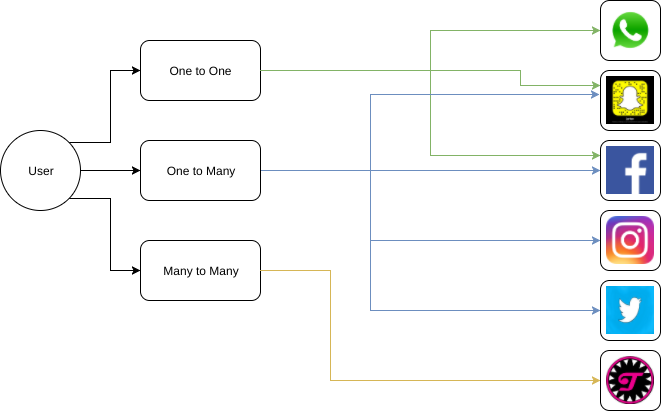
\includegraphics{similarServices}

	Talkatiel will be a Portable Web App, or a PWA.  This allows it to behave as an app does while also being much more accessible and easier to use for our end users.  The web app itself will consist primarily of 3 elements:   the service worker, the app shell, and the backend database.  A service worker is a chunk of code that exists outside the website.  It stays on a users device and works to cache and manage data for the web app.  It will also allow us to send push notifications to the user.  The app shell is the skeleton behind the web app.  It is stored on the users device, allowing the web app to load quickly.  It manages the basic user interface which is then filled with content from the server.  The database will store all posts along with identification and metadata information.

	Previously this idea has been attempted by Yik-Yak.  Originally released in 2013, Yik-Yak set out to solve many of the problems we are solving with Talkatiel.  One of the biggest issues that Yik-Yak encountered was bullying and harassment on the platform\cite{item1}.  The only moderation present in the app was an automod that deleted posts that had certain words.  This did not effectively deal with hurtful messages, only invited people to figure out better ways to circumvent the moderation.  To solve this, Talkatiel will use both word filtering and actual people to moderate.  As seen on sites like reddit, using trusted users to moderate other users can be a strong and effective tool.

	To build Talkatiel we will use Polymer for the user facing side.  It has been proven to be a simple and fast portable web app tool that allows us to quickly move from the idea stage to the testing stages of features.  Polymer is built on a mix of HTML, javascript, Node.js (4.x) and Bower.  The database will run on the google service FireBase.  This allows us to easily store and distribute user posts and settings and integrates easily with Polymer.  In addition to simply delivering data, Firebase also has extensive analytic and monitoring tools, allowing us to see the health of Talkatiel at a glance.

	We will be designing this for use primarily on mobile device browsers.  These include Chrome, Safari, and Firefox.  Because of the way PWA’s are structured, they should also perform well on desktop browsers such as Chrome, Edge, and Safari.

  Talkatiel will use a service worker to precache parts of a web app, allowing it to load quickly the next time the user uses it.  This allows us to manage what the user sees while cutting down on network traffic and load times.  A service worker can perform its tasks even when the web app isn’t open.  This means in addition to caching and managing web app data, it also has the ability to allow users to access things offline, intercept HTTP/HTTPS requests and even send push notifications to the user.
\subsection{Functional Requirements}
\subsubsection{Posting}
User will be able to create and post in discussions anonymously.  They will be able to read and respond to posts by other users.  Users will be able to reply to a discussion, reply to another reply and vote on posts.
\subsubsection{Moderation}
There will be both computer and real person moderation.  The computer run moderation will filter out posts will blacklisted words or phrases, while the human moderation will be done at the best judgment of whoever is moderating.
\subsubsection{Geolocation}
Users will only be able to post to certain discussions if they are with a range of the discussions marker.  If a user is within a certain distance they will be able to post to discussions.  If they are out of range of a discussion, they won’t be able to view or participate in the discussion.
\subsubsection{Viewing Posts}
Users will be able to scroll through posts made by others users.  They will be able to see the text of the post, and possibly how many votes the post has.  A user can then respond, vote, or continue scrolling to new content.
\subsubsection{Reporting}
Posts will be able to be reported for reason such as spam, abuse, bullying, or other issues.  These posts will then be dealt with by a human moderator, who can then choose to remove the post or let it be.  This will help cut out harmful speech that isn’t wanted on the platform.
\subsection{Non-Functional Requirements}
\subsubsection{Secure}
Talkatiel will need to utilize a secure connection (HTTPS).
All content needs to be delivered through a secure connection to confirm that all aspects of the app are controlled by us.  This tops malicious 3rd parties from abusing the service.
\subsubsection{Network Independent}
The app should still work when there is little or no network connectivity.
If not showing the different discussions, at least displaying a page notifying the user of the fact.  This will allow it to act as though it is a native app, though it is actually a website crafted for their device.  Also stops it from appearing "broken" to users, which could result in losing them.
\subsubsection{Responsive}
Talktatiel should be responsive to users on both phones and tablets.  The pwa should react quickly to user inputs, meaning that both the application presented to the user and the back-end database need to do their tasks speedily.
\subsubsection{Deep Linking}
Each page should have a distinct URL.  This means each discussion, post and reply should have it's own individual URL.  This allows user to share the post with others, such as on facebook or other social media services.
\subsubsection{Standard App Manifest}
Talkatiel should include a file that specifies all the metadata associated with it.
This allows us to set various settings for how the web app is displayed, such as orientation, display modes, image links, URL settings, and theming.  This is an integral part of making a portable web app and signals to browsers how to handle the website.
\subsection{Documentations}
In addition to a simple and intuitive user interface, there will also be a limited help section present.  It will show users how to do different basic functions of the application, such as navigating, posting, voting and the purpose.  The help section can walk a new user through the application and introduce them to the features.  By keeping the Talkatiel simple we can limit the amount of documentation needed while also improving user retention.
\subsection{Major Features}
\begin{itemize}
      \item Post text as part of discussion
      \item Reply to other user's posts
      \item Ability to vote up or down other posts
      \item Both computer and human moderation of posts
      \item Ability to participate and view discussions depending on location
      \item Ability to report posts to Moderators or Administrators
\end{itemize}
\subsection{Minor Feature / Strech Goals}
\begin{itemize}
      \item Ability to save discussions for later viewing.
      \item Ability for a user to view all of their own posts
      \item Keep track of the total votes a user has recieved
      \item Integrate ads into the platform
\end{itemize}
\section{Use Cases}

\begin{itemize}
  \item Use Case 1
  \item Use Case 2
  \item Use Case 3
\end{itemize}

\section{Planning}

\subsection{Milestones}
\subsection{Timeline}
\subsection{Project Tracking}
\subsection{Risk Management}


\section{Meeting Report}

\subsection{Progress Made This Week}
\subsection{Plans for Next Week}
\subsection{Team Member Contributions}
\subsection{Customer Meeting Status}

\newpage
  \begin{thebibliography}{1}

  \bibitem{item1} Lindsay Bramson {\em Yik Tak bullying leads district to ban app}  2014: KXAN.com. http://kxan.com/2014/09/29/yik-yak-bullying-leads-districts-to-ban-app/

  \bibitem{item2}  Nick Strayer {\em The Great Out-Of-State Migration: Where Students Go} 2016:
  New York Times. https://www.nytimes.com/interactive/2016/08/26/us/college-student-migration.html

  \end{thebibliography}

\end{document}
